\chapter{Example Scenario} \label{ch:example}

The paper presented in Chapter \ref{ch:paper1} was written before the workload concepts and modeling language semantics had settled into their current form.  Jared et al. \cite{moore2014modeling}, in concert with this work, published a paper that expands on the concepts in Chapter \ref{ch:paper1} but is also slightly outdated.  Thus we feel it expedient to summarize those aspects of the language which are critical to our metrics before we present the metrics themselves.  To assist in this effort we have prepared a simple scenario which includes a partial model and illustrations of the DiTG, and labeled state transition system.

\section{Example Scenario}
In this scenario there are two people, Alice and Bob.  Alice is standing next to Bob listening to a friend on her cell phone.  Bob suddenly remembers that he wants to ask Alice out.  Not noticing that Alice is listening to her phone Bob starts to ask Alice on a date.  When this happens Alice looks at Bob and points to her phone, signaling to him that she is on the phone.  Bob stops talking and decides between waiting for her to finish or walking away.  Eventually Bob walks away.

\subsection{Actors}
From the scenario above we create three Actors: A) Alice, B) Bob, and C) Cell Phone.  Actors represent any aspect of the system that has state.  An Actor can be anything.  In our example we have two humans and a cell phone.  We could also create a sub-Actor which is part of a larger Actor, such as Bob's hair, and give it states like messy or combed.  Actors can also be very abstract or very detailed.  The more states an Actor contains, the more expressive it becomes.

\begin{figure}[h]
\begin{center}
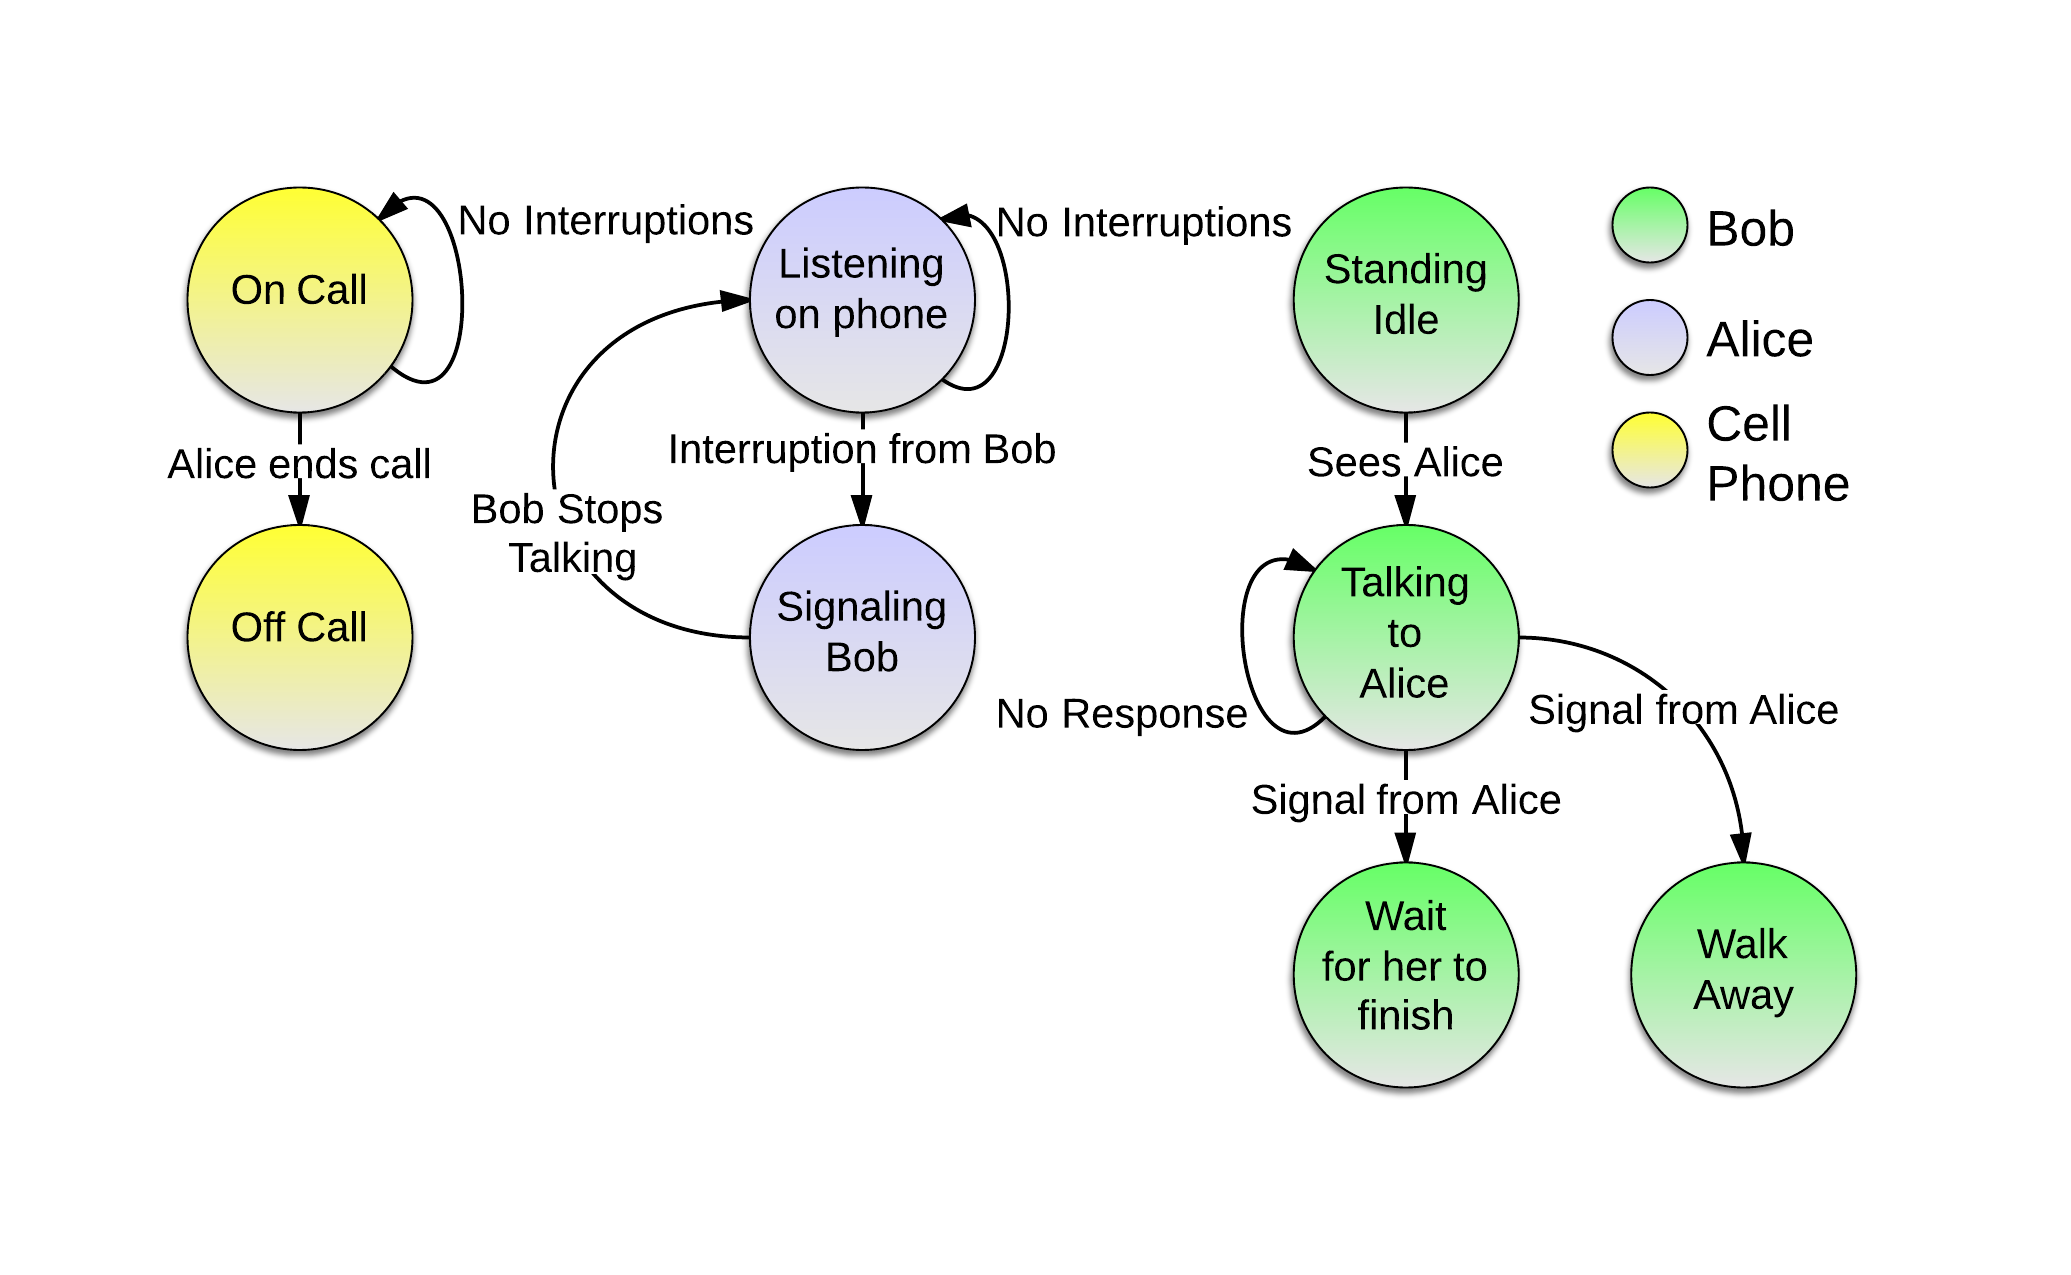
\includegraphics[width=\textwidth]{ab_dirg.png}
\caption{State Transition System for Alice and Bob scenario}
\label{fig:ab_dirg}
\end{center}
\end{figure}

While we ultimately express an Actor as a labeled state transition system, for now we describe the Actors as simple state transition systems.  The state transition system represents how an Actor is allowed to flow between states and can be visualized as a directed graph.  Figure~\ref{fig:ab_dirg} represents all three Actors as a state transition system.  We see that Alice is initially in a {\em Listening on phone} state while Bob is in the {\em Standing idle} state.  Alice can either stay in the {\em Listening on phone} state, shown by the looping transition, or move into the {\em Signaling Bob} state.  Once in the {\em Signaling Bob} state her only choice is to stay there forever or to return to the {\em Listening on phone} state.  We see from figure \ref{fig:ab_dirg} that Alice and Bob are interacting with one another and influencing the transitions of the other.  To define the characteristics of the transitions we convert our state transition system into a labeled state transition system, however, before we do so must first define the inter-Actor relationship that allows Actors to influence one another.


\subsection{Channels}
We define inter-Actor connections as Channels.  A channel is a uni-directional communication medium which allows an Actor to send information to another Actor.  Each Channel is composed of a source Actor, a target Actor, and a type.  The source Actor sends information as {\em output}, the target Actor receives the information as {\em input}, and the type specifies which communication medium is being used.  When describing the metrics we sometimes refer to the Channel source as the input source and the Channel target as the output target.  In the case of Alice and Bob we use audio, visual, and manual Channels~\cite{wickens2002multiple}, the case study in Chapter \ref{ch:UASinNAS} also uses a Data channel that represents network communication.  

We also designate that each Channel can represent multiple layers of communication.  To show this we will use the visual channel from Alice to Bob as an example.  We can express Alice's {\em output}, Bob's {\em input}, as two different layers on the visual channel, one for Alice's body language, and another for her facial expressions.  This allows us to explicitly set how much data is being sent over the channel, it also allows us to express multiple visual inputs for Bob without creating a {\em channel conflict}.  A {\em channel conflict} occurs when an Actor is receiving input from two or more channels of the same type.  In our example scenario Alice is listening to her cell phone which uses an audio channel.  At the same time Bob is talking to Alice on a different audio channel.  Because Alice is receiving {\em input} on multiple audio channels she has an audio channel conflict.  

\begin{figure}[h]
\begin{center}
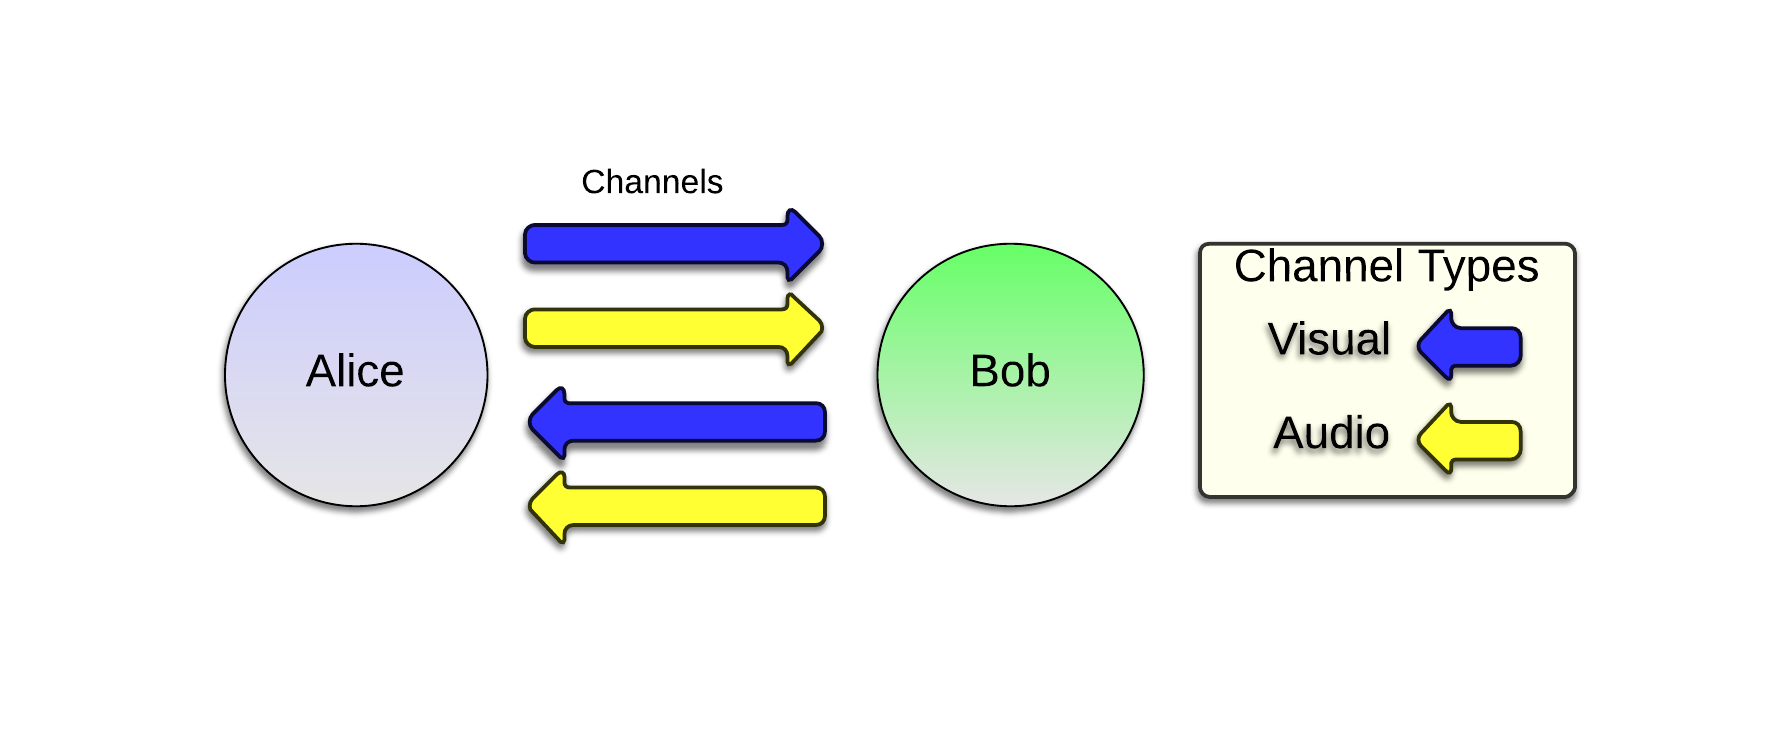
\includegraphics[width=\textwidth]{ab_ditg.png}
\caption{Directed Team Graph for Alice and Bob scenario}
\label{fig:ab_ditg}
\end{center}
\end{figure}

\subsection{DiTG}
To express a systems Channels we use a Directed Team Graph (DiTG)\cite{moore2014modeling}.  The DiTG defines all the channels that exist between the Actors within the system.  Figure \ref{fig:ab_ditg} shows the DiTG for our Alice and Bob scenario.  From the figure we can see that Alice has two channels to Bob, an audio and a visual and an audio channel to her cell phone.  We also see that Bob has two channels to Alice, an audio and a visual.  Lastly, the cell phone has an audio channel to Alice.  While the simplicity of this scenario makes it difficult to see the value of the DiTG, by combining the DiTG with the state transition system we have effectively constrained the Actor behavior and communication for the entire system.  With the constraints in place we are ready to define the behavior of the system, which we do with transitions.


\subsection{Transitions}
Transitions represent an Actor's behavior.  Transitions tells us about the state of the Actor, what caused the Actor to change state, and how that change effects the system.  Transitions are composed of a start state, an end state, a set of input equations, a set of outputs, a duration, and a priority.  The Transition start and end states represent two Actor states and signifies that the Actor can move from the start state to the end state.  

The Transition input equations are used to determine if the transition is enabled.  Each equation is composed of a source value, a predicate, and an expected value.  The source value is obtained from one of two sources, Channels or Memory.  Actor memory is an internal variable that allows an Actor to store and retrieve data.  For predicates we use equal to, less than, greater than, etc.  The structure of the input equations allows each equation to evaluate to a simple true or false.  If all input equations evaluate to true then the Transition is enabled.  

The Transition outputs contain all output generated by the transition as a set of target value pairs.  The target is the Channel or Memory variable that will receive the designated value.  The Transition duration is a range which represents the minimum and maximum number of time steps that a transition will remain {\em active} before it {\em fires}.  When an Actor decides to transition it selects an enabled transition to become {\em active}.  While a Transition is {\em active} its outputs are kept in temporary memory stored by the Simulator, once the Transition {\em fires} the Actor changes state and the temporary outputs are sent to the respective channels.  We sometimes refer to inputs and outputs as being {\em active}, this implies that they are coming from an {\em active} Transition and that the value is not null.  The final Transition element is priority.  Priority reflects how important a Transition is to the Actor relative to the other Transitions.  If multiple Transitions are enabled the Actor will choose the Transition with the highest priority.

\begin{figure}[h]
\begin{center}
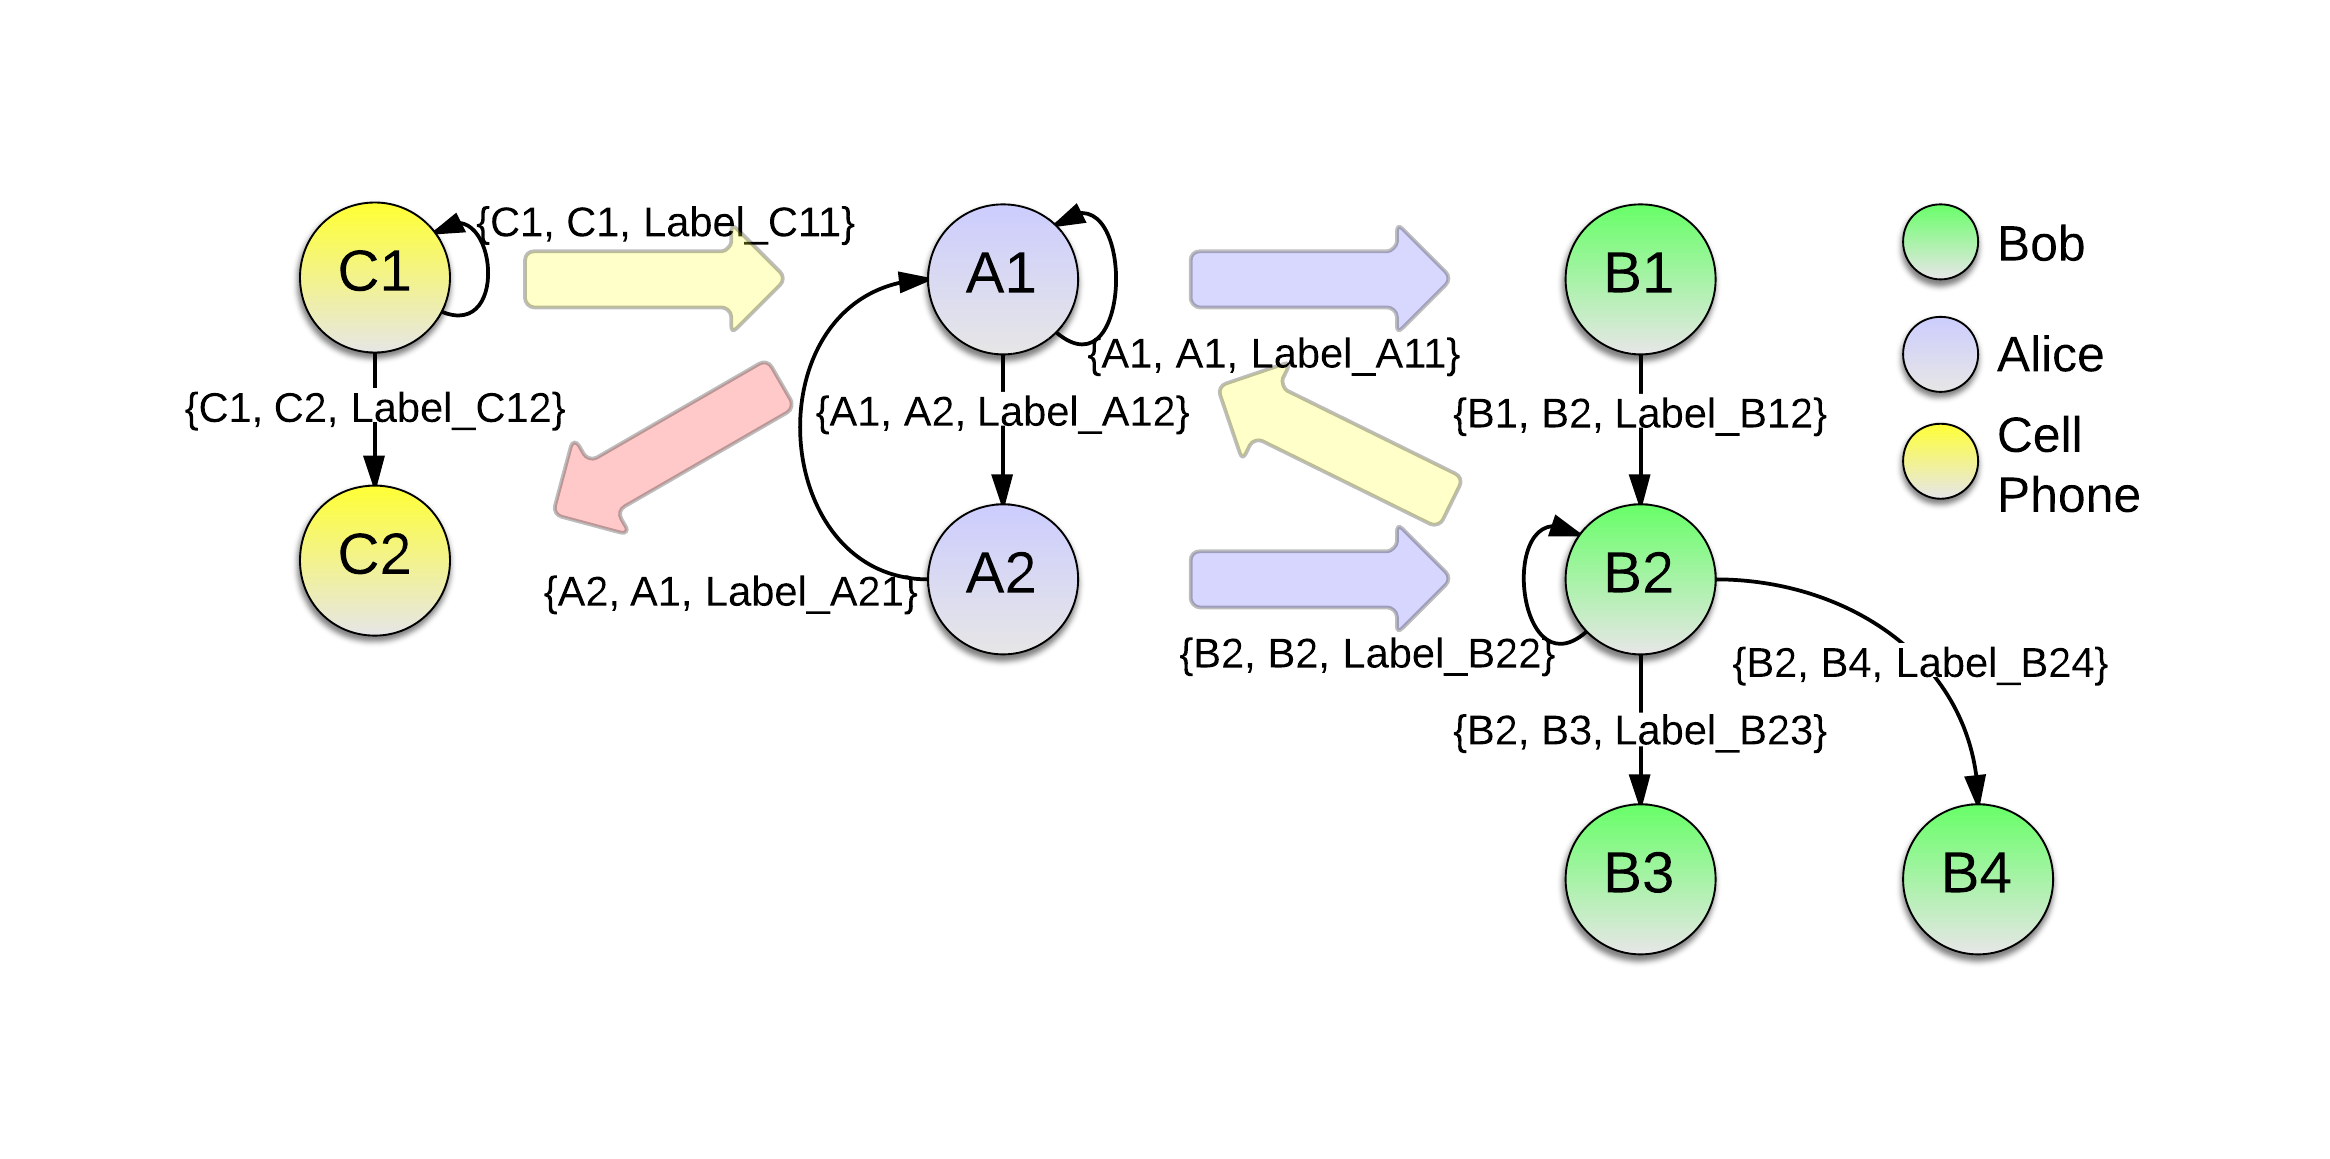
\includegraphics[width=\textwidth]{ab_lsts.png}
\caption{Labeled State Transition System for Alice and Bob scenario}
\label{fig:ab_lsts}
\end{center}
\end{figure}

\subsection{Labeled State Transition System}
The inclusion of the transition properties represent the switch from a state transition system to a labeled state transition system.  In our case the label translates directly to the transition input equations, outputs, duration, and priority.  The label allows us to determine if a transition is enabled, if it should be fired, how long it remains active, what outputs it sends out and more.  

In figure \ref{fig:ab_lsts} we can see that every transition has a label.  These labels are used by the simulator to determine if the transition is enabled, what channels will become {\em active}, and how long those channels should remain {\em active} before the state changes.  To make this clear we will describe $Label_A12$ of Alice's transition from the {\em Listening on phone} state to the {\em Signaling Bob} state.  From figure \ref{fig:ab_lsts} we see that when Bob is speaking to Alice there is an audio channel that is {\em active} (opaque yellow arrow).  The description on the transition implies that Bob's talking has somehow triggered the transition, to represent this in the label we create two input equations.  Audio channel from Bob does not equal null.  And audio channel from Cell Phone does not equal null.  This means that when Alice is listening to her cell phone if she hears Bob at the same time then this transition becomes enabled.  If she chooses to follow the transition then the transition becomes {\em active} and the transition outputs will become active.  In this case the output is a signal on the visual channel from Alice to Bob.  We will make the duration 5 seconds with a priority of 1.  

The XML language we developed allows us to model scenarios using the concepts summarized in this chapter.  Using our XML parser, appendix \ref{ch:xmlparser}, the model is converted into the Java classes used by the Simulator to generate and execute a labeled state transition system.  We chose the labeled state transition system because the state transition system lends itself well to model checking while the label allows us to add data points that relate specifically to workload.  Almost all of the label values are present in the workload metrics that we present next.

